\chapter{Theory}
\section{Bloch Wave}\label{sec:bloch}
\textbf{Theorem} (without proof) Let $V:\mathbb{R}^3\longrightarrow\mathbb{R}$ denote a scalar potential obeying periodic boundary conditions, such that $V(\mvec{r}) = V(\mvec{r}+s\cdot\mvec{T})$, where $s\in\mathbb{Z}$ and $\mvec{T}$ is the translation vector of a periodic lattice. Then, the stationary Schrödinger equation has solutions, which satisfy $\psi_k(\mvec{r}+\mvec{T}) = \e^{i\mvec{k}\cdot\mvec{T}}\cdot\psi_k(\mvec{r})$, where $\psi_k(\mvec{r})$ is a solution of the non-periodic stationary Schrödinger equation with a wave vector $\mvec{k}$.

\textbf{Remark} Such solutions are called \textit{Bloch waves}. The electron wave functions in a crystal lattice have a basis consisting entirely of Bloch wave energy eigenstates. This is easy to see, if one introduces a translation operator $\hat{T}$, such that $\hat{T}\psi (\mvec{r}) = \psi (\mvec{r}+\mvec{T})$. For a periodic potential, $\hat{T}$ commutes with the Hamiltonian, because the crystal has translational symmetry. Therefore, there is a simultaneous eigenbasis of the Hamiltonian and every possible translation operator (note that $\comm{T_i}{T_j} = 0$ for every $i\neq j$).
The eigenstates in this basis are energy eigenstates and Bloch waves at the same time.

\section{Electronic Band Structure}
If the electronic configuration inside of a periodic lattice is approximated as being free, according to the stationary Schrödinger equation for electrons, an electronic dispersion relation of
\begin{equation*}
	E(k) = \frac{\hbar^2 k_n^2}{2m},
\end{equation*}
is obtained, where the possible wave vectors $k_n = n\cdot\frac{\pi}{a}$ are determined by periodic boundary conditions.
$a$ denotes the lattice parameter.
This means that the dispersion relation for free electrons inside the lattice is periodically parabolic.

\begin{figure}
	\centering
	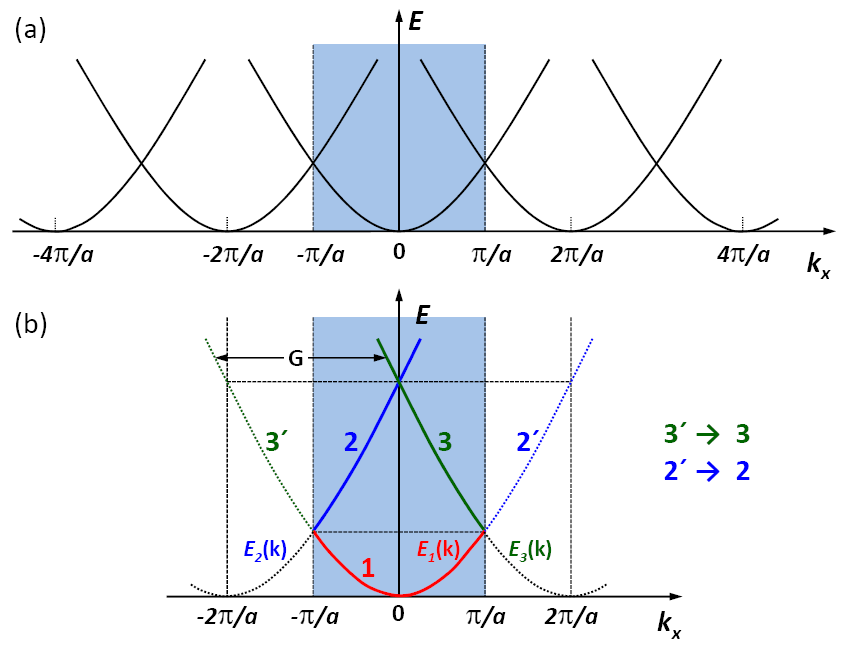
\includegraphics[width=.6\textwidth]{./img/reducedzone.png}
	\caption{Reduced zone scheme, obtained by mirroring the dispersion relation into the first Brillouin zone\\ Source: \cite{graz}}
	\label{fig:reducedzone}
\end{figure}
The periodicity can be translated into the reduced zone scheme by mirroring (as depicted in \autoref{fig:reducedzone}).
However, at the edges of the first Brillouin zone, the electrons satisfy the Bragg condition and are therefore mirrored to the opposite side of the first Brillouin zone.
This leads to the creation of standing waves in k-space at both zone edges.
For a periodic potential generated by the nuclei in the lattice, the electron probability density is able to snap into the lowest energy solutions in two different ways:
\begin{itemize}
\item \textbf{Maxima of $|\psi|^2$ at locations of nuclei:} As a consequence of the tight Coulomb binding between the electrons and nuclei, the energy is lowered with respect to the free parabolic dispersion. The parabola is bending downwards.
	\item \textbf{Maxima of $|\psi|^2$ between locations of nuclei:} Illustratively speaking, the electrons are located further away from the nuclei. Hence, the energy is raised with respect to the free parabolic dispersion as a consequence of the looser Coulomb binding. The parabola is bending upwards.
\end{itemize}

In total, the parabola bends cause the band structure by introducing a \textit{band gap}.
Electronic states which lie inside the band gap are forbidden.
The resulting bands are now filled up, considering the Pauli exclusion principle.
At \SI{0}{\kelvin}, there are no electrons with energies above the Fermi energy $E_\text{F}$.
At room temperature, however, some electrons are thermally excited into states above the Fermi energy, since the Fermi distribution
\begin{equation*}
  \overline{n_\lambda} = \frac{1}{\e^{\beta\left(\epsilon_\lambda-\mu\right)} + 1}
\end{equation*}
is only approaching a Heaviside theta function for $T\rightarrow 0$.
$\overline{n_\lambda}$ and $\epsilon_\lambda$ denote the mean particle density and the energy of state $\lambda$ respectively, $\mu$ is the chemical potential and $\beta=\frac{1}{k_\text{B}T}$.
Depending on the filling of these bands, a distinction is made between
\begin{itemize}
	\item \textbf{isolators:} valence band full, conduction band empty, large band gap,
	\item \textbf{semiconductors:} valence band full, conduction band empty, small band gap,
	\item \textbf{metals:} valence band full, conduction band partially full.
\end{itemize}

\section{Semiconductors}
Semiconductors are materials with a Fermi level inside their band gap at equilibrium, where the band gap is significantly smaller than that of an insulator.
Depending on the size of the band gap,
\begin{itemize}
	\item \textbf{narrow gap semiconductors}, with $0<E_\text{g}\leq\SI{0.5}{\eV}$,
	\item \textbf{ordinary semiconductors}, with $\SI{0.5}{\eV}<E_\text{g}\leq\SI{2}{\eV}$ and
	\item \textbf{wide gap semiconductors}, with $E_\text{g}\geq\SI{2}{\eV}$
\end{itemize}
are distinguished theoretically.
In practical use cases, the distinction between insulators (with $E_\text{g}\geq\SI{4}{\eV}$) is loosen up depending on the context.
For example, diamond ($E_\text{g}\approx\SI{5.5}{\eV}$) is still considered to be an ordinary semiconductor.

Two types of semiconductors may be distinguished: intrinsic semiconductors which have their Fermi level right in the middle of the band gap and extrinsic semiconductors which are also referred to as 'doped'. The Fermi energy of doped semiconductors is dependent on their doping concentration. It can be shown that, depending on the doping type, the Fermi energy obeys
\begin{align*}
	E_\text{F,n} &= E_\text{i} + k_\text{B}T\log\frac{n}{n_\text{i}} \\
	E_\text{F,p} &= E_\text{i} - k_\text{B}T\log\frac{p}{n_\text{i}},
\end{align*}
where $E_\text{i}$ and $n_\text{i}$ denote the instrinsic (undoped) Fermi energy and density respectively ($n$ and $p$ explained in \autoref{sec:cc})

\subsection{Doping}
A pure semiconductor is not very useful, since it is neither a good insulator, nor a good conductor.
By adding impurities to or gating pure semiconductors (such as pure Si) their electrical properties may be varied in a useful manner.
Doping and gating draw either the conduction or the valence band very close to the Fermi level, greatly increasing the number of free states there.

Doping is accomplished by adding small quantities of foreign atoms to the semiconductor.
Consider for example Si from the fourth main group of the periodic system of elements which has four valence electrons that bond each silicon atom to its neighbors.
Adding either elements from the third (i.e. B, In) or fifth main group (i.e. As, P) may be used for creating p- or n-doped semiconductors, since they either lack or add one electron in their valence shells.

In \textit{p-doped} materials the so called \textit{acceptors} leave a vacant electron state (\textit{hole}) when they replace a silicon atom in the crystal.
This hole can move around the lattice and function as a charge carrier.
The acceptor levels have energies just above the valence band.
By supplying a small amount of energy, electrons from the valence band may be excited into these acceptor states and thus ionize the foreign atom, leaving a negatively charged defect behind.

Similarly, in \textit{n-doped} materials the so called \textit{donators} leave one electron free, which can contribute to the conductivity of the material.
These weakly bound electrons have energies just below the conduction band and thus can be excited very easily into conducting states by supplying a small amount of energy.

Electrons and holes are characterized by their \textit{effective masses}.
Consider wave packets as a superposition of Bloch states, moving with a group velocity of
\begin{equation*}
	v_\text{g} = \frac{1}{\hbar}\pdb{E}{k}.
\end{equation*}
Calculating $a=\pdb{v_\text{g}}{t} = \frac{F}{m}$, the concept of effective can be introduced as
\begin{equation*}
	m_\text{eff}^{-1} = \frac{1}{\hbar^2}\frac{\partial E}{\partial k_i \partial k_j},
\end{equation*}
which implies that $m_\text{eff}$ has tensor qualities.

\section{Carrier Concentration in Non-Degenerate Semiconductors}\label{sec:cc}
Assuming that the Fermi energy of a semiconductor lies far within the band gap, Fermi-Dirac statistics may be replaced by Boltzmann statistics, effectively treating the electrons as a classical gas.
This approximation is called the \textit{non-degenerate approximation} and may only be used, if the Fermi energy is located far enough away from both band edges with respect to the thermal energy $k_\text{B}T$ of the system.

In the non-degenerate approximation, the carrier concentrations
\begin{align*}
	n &= \int_{E_\text{c}}^\infty\d E\ \nu_\text{n}(E)\cdot\e^{-\frac{E-E_\text{F}}{k_\text{B}T}} \\
	p &= \int_{-\infty}^{E_\text{v}}\d E\ \nu_\text{p}(E)\cdot\e^{-\frac{E_\text{F}-E}{k_\text{B}T}}
\end{align*}
can be calculated analytically and be used to calculate intrinsic carrier concentration with the condition $n=p$ as
\begin{equation*}
	n_\text{i}(T) \propto T^{\nicefrac{3}{2}}\cdot\e^{-\frac{E_\text{G}}{2k_\text{B}T}}.
\end{equation*}
$\nu_\text{n/p}$ denote the density of states for electrons and holes respectively. $E_\text{c/v}$ are the conduction/valence band energies.

Taking the logarithm on both sides and rearranging yields a way, to determine the band gap energy $E_\text{G}$
\begin{equation*}
	\log{\frac{n_\text{i}}{T^{\nicefrac{3}{2}}}} = \log{A} - \frac{E_\text{G}}{k_\text{b}T},
\end{equation*}
by plotting the LHS against $\frac{1}{T}$. This is called an \textit{Arrhenius plot}.

\section{Classical Electrical Conductivity}
The classical concept of free, localized electrons gives a simple explanation for electrical resistance, assuming that the electrons can scatter on the nuclei of the conductor material.
An external electric field $E$ accelerates the electrons with mass $m$, which regularly lose their kinetic energy to elastic collisions with nuclei.
The mean time between collisions $\tau$ depends on the parameters of the conductor's lattice structure.
Solving the equations of motion gives the term
\begin{equation*}
	v_\text{D} = - \frac{e \tau}{m} E = - \mu E
\end{equation*}
for the mean drift velocity $v_\text{D}$ and serves as the definition of the mobility $\mu$.
The current density $j$ is given by $j = - e n v_\text{D}$, where $n$ denotes the density of charge carriers.
Using the definition of the conductance $j = \sigma E$ yields
\begin{equation}\label{eq:classical-resistance}
	\sigma = \frac{n e^2 \tau}{m} = e n \mu.
\end{equation}

\section{Charge Carrier Mobility}
Expanding on the drude model of electrical conductivity, it has been discovered that electrons do not scatter on a periodic grid of nuclei as the wave functions are superpositions of time-independent bloch waves.
Scattering only occurs at defects, different kinds of which give different dependencies on temperature.

\subsection{Scattering on Charged Defects}\todo{Bild zum mu-Verlauf}
Electrons scatter on the coulomb potential of charged lattice defects, such as atoms introduced for doping semiconductors.
This process is described in classical Rutherford scattering, where the cross section relates to the velocity of the incoming electron as $\sigma_\text{Ru} \propto v^{-4}$.
Using the classical velocity distribution $^1/_2 m v^2 = {^3}/_2 k T$ gives the relations $\sigma_\text{Ru} \propto T^{-2}$ and $\tau \propto \frac{1}{\sigma_\text{Ru} v} \propto T^{{^3}/_2}$.

\subsection{Scattering on Phonons}\label{subsec:phonons}
There is an important distinction to be made between monoatomic and compound semiconductors, the latter of which have ionic bindings between lattice points.
This means that there is a net charge movement for phonons of the optical branch and present an additional source of coulomb scattering or, in this context, 'polar' scattering.

\textbf{Acoustic phonons} add a source of both polar and non-polar scattering, which both depend on temperature as $\tau \propto T^{-{^3}/_2}$.
In the special case of a 2DEG, the dependence changes to $\tau \propto T^{-1}$.

Both polar and non-polar scattering on \textbf{optical phonons} only depend on the number of phonons.
It holds $\tau \propto \e^\frac{\hbar \omega}{k T} - 1$, where $\omega$ denotes the angular frequency of the phonon.

\subsection{Total Mobility}
The scattering rates of the individual processes add up, so the relaxation times $\tau_i$ combine as $\tau_\text{total}^{-1} = \tau_1^{-1} + \tau_2^{-1} + \dots$.
As $\tau \propto \mu$, this also applies to the total mobility.

Only the total mobility can be determined experimentally, but the different dependencies on temperature allow the quantification of the contributions of the individual processes.

\section{Van-der-Pauw Method}\label{sec:van-der-pauw-geometry}
Manufacturing samples with the very precise geometries required for experiments is an experimental challenge.
To obtain accurate results even with imperfect samples, the Van-der-Pauw method is used.
This method allows measuring the sheet resistance of a sample of constant thickness and otherwise arbitrary shape.
Four point-like contacts are placed on the sample and the resistance between pairs of points is measured with a four-wire method.
The points are numbered in a circular fashion.
A current is applied between two points (ex. 1 and 2) and the voltage between the other two points (ex. 3 and 4) is measured.
This yields the resistance $R_{12,34} = \frac{U_{34}}{I_{12}}$.

Van-der-Pauw proved theoretically that for such a measurement, two resistances between three adjacent points relate to the sheet resistance $R_\text{s}$ of the sample as
\begin{equation}
	\e^{- \uppi \; ^{R_{12,34}}/_{R_\text{s}}} + \e^{- \uppi \; ^{R_{23,41}}/_{R_\text{s}}} = 1.
\end{equation}
There exists no analytical solution, so $R_\text{s}$ can only be approximated numerically.

Assuming a roughly square sample ($R_{12,34} \approx R_{23,41}$), the sheet resistance approximates
\begin{equation*}
	R_\text{s} = \frac{\uppi}{\ln 2} \cdot \frac{1}{2} \left( R_{12,34} + R_{23,41} \right).
\end{equation*}
The specific conductivity of a sample with finite thickness $h$ is calculated as $\sigma = \frac{h}{R_\text{s}}$.

The hall coefficient $R_\text{H}$ is obtained by measuring the resistance across the sample (eg. $R_{13,24}$), instead of along the edges.
It holds
\begin{equation*}
	R_\text{H} = \Updelta R_{13,24} \cdot \frac{h}{B_\text{v}},
\end{equation*}
with the magnetic field perpendicular to the sample $B_\text{v}$ and the difference of resistances $\Updelta R_{13,24}(B = B_\text{v}) - R_{13,24} = R_{13,24}(B = 0)$.
